\documentclass[a4paper,10pt,fullpage]{report}
\usepackage[fontsize=14]{fontsize}
\usepackage{setspace}
\setstretch{1.5}
\usepackage[top=2.5cm,bottom=2.5cm, left=2.5cm, right=3cm]{geometry}
\usepackage{sectsty}
\sectionfont{\fontsize{14}{16}\selectfont}
\subsectionfont{\fontsize{14}{16}\selectfont}
\usepackage{indentfirst}
\setlength\parindent{1cm}
\usepackage{tocloft}
\renewcommand{\cftchapdotsep}{\cftdotsep} % dotted chapter leaders


%\renewcommand{\cftsecleader}{\cftdotfill{\cftdotsep}} % for sections
\usepackage{titlesec}
\usepackage{afterpage}
\usepackage{caption}

\captionsetup{
	font=small
}

\usepackage{import}
\usepackage{graphicx}

 %\usepackage[a4,frame,center,noinfo]{crop}
\usepackage{longtable}

\usepackage{array}
\usepackage{subfiles}
\usepackage{blindtext}
\usepackage{booktabs}
\usepackage{supertabular}
\usepackage{float}
\usepackage[section]{placeins}

\usepackage{titletoc}



\usepackage{subfig}
\usepackage{xr}
\usepackage{multirow}


\usepackage{hyperref}
\hypersetup{
	colorlinks=true,
	linkcolor=blue,
	filecolor=magenta,      
	urlcolor=cyan,
	citecolor=cyan
}

\usepackage{amsmath}
\usepackage{amssymb}
\usepackage[fleqn]{mathtools}
\usepackage[ruled, vlined]{algorithm2e}
\usepackage{tablefootnote}

\usepackage[table]{xcolor}
\usepackage[noadjust]{cite} 


\usepackage{xepersian}
\settextfont{XB Niloofar}
\setlatintextfont{Times New Roman}
\renewcommand{\thesection}{\thechapter-\arabic{section}}
\renewcommand{\thesubsection}{\normalsize{\thesection-\arabic{subsection}}}
\renewcommand{\thesubsubsection}{\normalsize{\thesubsection-\arabic{subsubsection}}}
\renewcommand{\thefigure}{\thechapter-\arabic{figure}}
\renewcommand{\thetable}{\thechapter-\arabic{table}}
\renewcommand{\theequation}{\thechapter-\arabic{equation}}
\renewcommand{\bibname}{منابع}


\titleformat{\chapter}[display]
{\bfseries \huge \centering}
{\bfseries \huge\chaptertitlename\ \tartibi{chapter}}
{6cm}
{\vspace{0.5ex}}
[\vspace{0.5ex}]


\renewcommand{\labelitemi}{$\bullet$}
\renewcommand{\labelitemii}{$\circ$}
\newcommand{\comment}[1]{}
\newcommand{\pluseq}{\mathrel{+}=}
\newcommand{\subeq}{\mathrel{-}=}

\newcommand{\PreserveBackslash}[1]{\let\temp=\\#1\let\\=\temp}
\newcolumntype{L}[1]{>{\PreserveBackslash\raggedleft}p{#1}}
\newcolumntype{C}[1]{>{\centering\centering}p{#1}}
\newcolumntype{R}[1]{>{\PreserveBackslash\raggedright}p{#1}}


\title{
\vspace{-4cm}
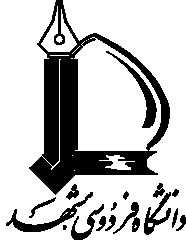
\includegraphics[width=1.24in, height=1.5in]{img/fum_logo_black.png}\\
\fontsize{14}{15}\selectfont
دانشکده مهندسی \\
\fontsize{12}{13}\selectfont
گروه مهندسی صنایع\\
\vspace*{\baselineskip}
\fontsize{16}{17}\selectfont
	پایان‌نامه کارشناسی ارشد\\
\vspace*{1\baselineskip}
\fontsize{20}{21}\selectfont
\textbf{عنوان}
}

\author{
	\begin{minipage}{\textwidth}
		\vspace*{1\baselineskip}
		\centering
		\fontsize{14}{15}\selectfont
		\textbf{استاد راهنما}\\
		\textbf{نام استاد راهنما}
		\vspace*{1\baselineskip}
		\linebreak \textbf{نگارش}\\
			\textbf{نام دانشجو}
	\end{minipage}
}



\date{
\fontsize{14}{15}\selectfont
\vspace{3cm}
\textbf{شهریور ۱۴۰۲}
}




\begin{document}
	\renewcommand{\bibname}{منابع}
	\newgeometry{left=3cm,right=3cm}
	
	\maketitle
	
	\restoregeometry
	\pagenumbering{alph}
	\chapter*{}
	 صورت جلسه دفاع
	 \chapter*{}
	 اظهارنامه
	 \chapter*{}

	 	  \textbf{\large{تقدیم به،}}


	   	 \begin{center}

	   \end{center}
	   
	\vspace{-3cm}
\chapter*{\large{تشکر و قدردانی}}



	\newgeometry{top=2.5cm, bottom=2.5cm, outer=2.5cm,inner=3cm}
	\vspace{-3cm}
	 \chapter*{چکیده}
	\addcontentsline{toc}{chapter}{\numberline{} چکیده}
	متن چکیده
	\\ \\
	\textbf{کلیدواژه‌ها:}

	
	\section*{}
	\addcontentsline{toc}{chapter}{\numberline{} فهرست مطالب}
	\vspace{-3cm}
	\tableofcontents  
	\pagebreak
	
	\section*{}
	\addcontentsline{toc}{chapter}{\numberline{} فهرست جداول}
	\vspace{-3cm}
	\listoftables
	\pagebreak
	
	\section*{}
	\addcontentsline{toc}{chapter}{\numberline{} فهرست تصاویر}
	\vspace{-3cm}
	\listoffigures{}
	\pagebreak
	
	\pagenumbering{arabic}

	\chapter{ کلیات پژوهش}
		متن فصل....
یک فرمول:
\begin{align}
\sum x_t \geq D_t
\label{eq1}
\end{align}

اشاره به فرمول \eqref{eq1} ...

متن انگلیسی را نیز می‌توان به کمک \lr{lr} نوشت.

اشاره به منبع: \cite{wood_ethereum_nodate}
 

	
	\chapter{مبانی نظری و پیشینه پژوهش}

	\chapter{روش پژوهش}


	\chapter{حل مدل و تجزیه و تحلیل یافته‌ها}


	\chapter{نتیجه‌گیری و پیشنهادات}


	\pagebreak
	
	\addcontentsline{toc}{chapter}{پیوست‌ها}
	\appendix
	\chapter{عنوان}

	\addcontentsline{toc}{chapter}{\numberline{} منابع}	
	\bibliographystyle{ieeetr-fa}
 	\bibliography{mylibs}




\begin{latin}
	\chapter*{Abstract}
	 \thispagestyle{empty} 6
	\addcontentsline{toc}{chapter}{\numberline{}Abstract}
	Write English Abstract...

	\textbf{Keywords:} Keyword1,..
\end{latin}
\pagebreak

\begin{center}
	\pagenumbering{gobble}
\title{
	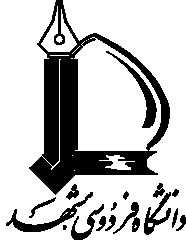
\includegraphics[width=1.24in, height=1.5in]{img/fum_logo_black.png}\\
	\fontsize{14}{15}\selectfont
	\lr{Ferdowsi University of Mashhad}\\
	\fontsize{12}{13}\selectfont
	\lr{Faculty  of Engineering } \\
	\vspace*{\baselineskip}
	\fontsize{16}{17}\selectfont
	\lr{MSc Thesis}\\
	\vspace*{2\baselineskip}
	\fontsize{20}{21}\selectfont
	\textbf{\lr{Sustainable Supplier Selection and Order Allocation using Blockchain}}
	\\
	\vspace*{2\baselineskip}
}
\author{
	\fontsize{14}{15}\selectfont
	\lr{\textbf{By:}}\\
	\lr{\textbf{Shayan Sadeghi}} \\
	\vspace*{\baselineskip}
	\lr{\textbf{Supervisor:}} \\
	\textbf{\lr{Dr. Mohammadali Pirayesh}}
	
}
\date{
	\fontsize{14}{15}\selectfont
	\vspace{\fill}
	\lr{September 2023}
}


\end{center}

\end{document}
